\chapter{Appendix}\label{chapter:Appendix}

\section{Additional Details to LRP Rules and CRP Implementation}
\label{appendix:lrprules}
\begin{itemize}
    \item explain used LRP rule \textit{epsilon plus flat} in sufficient detail
    \item explain what canonizers are and why they are not necessary for my example (model is simple and does not have batch norm layers) 
    \item additional information on implementation and theoretical background of CRP?
    
\end{itemize}
\subsection{Interpretation Techniques from CRP Work}
The authors of CRP embed the approach into a handful of concept-based interpretation techniques. Their motivation is to gain more abstract, reduced explanations, while still potentially using multiple concepts. The underlying assumption is that the neurons in layers of deep neural networks encode human-understandable concepts hierarchically from low-level to abstract \cite{Zeiler2013,Bau2017,Olah2017}. Although this assumption seems to be made mostly for large and deep CNN and complex image datasets, the general idea can be applied in our experiment too. 

\subsubsection{Relevance Maximization}
Prominently, they introduce \textit{Relevance Maximization}, creating reference sets of images for all neurons encoding potentially human-understandable concepts. It is the \textit{relevance} analogue to \textit{activation maximization} \cite{Nguyen2016}. This technique arguably reduces the complexity of the explanation as \textit{learning-by-example} is proven to be a prevailing human strategy.
Therefore it seems fair to evaluate feature importance based on those reference sets. If a set overlaps strongly with regard to the spurious feature's value, one can assume this feature to be the concept encoded by that concept/neuron. 
Unfortunately the overlap of our feature of interest might be disguised by other features. As an example: while each image in a set might have the watermark, they might all show the same shape in a similar rotation too. This indeed happens with our benchmark dataset (see \cref{fig:suppressor_ref}), probably also because of its generally low complexity. 

\begin{figure}
    \centering
    \includegraphics[width=0.3\textwidth]{thesis_latex_template/pics/suppressed_reference_set.png}
    \caption[Reference Set Interpretation]{Example of a reference set, with unclear interpretation}
    \label{fig:suppressor_ref}
\end{figure}

\section{Details on Adapted dSprites Datasets}\label{appendix:dsprites}

The generating factors \verb|shape|, \verb|scale|, \verb|rotation|, \verb|x-position| and \verb|y-position| are known for each of the 437'280 samples. 
To adapt the benchmark for our purpose, only the first two shape classes (rectangle and ellipse) are used. 
Initially we added watermark in the form of a small \textit{w} to the lower-left corner of the images. During first experiments with only this adaptation it became clear that even the small convolutional neural network employed here is too powerful for this kind of task, as effectively dividing the image into two parts solves the problem and most neurons became irrelevant.
To make the spurious feature, which is the watermark \textit{w}, more difficult to learn, its position is varied across the edges of the image. Further, a small Gaussian noise term is added to make the samples closer to realistic images and harder to learn. The other latent factors are not a part of our analysis although the dataset was initially created to test disentanglement of such factors. Nonetheless, a comparison of the importance of other factors with the used factor shape might give an impression of the overall ability of a model to disentangle them. It could also serve as a baseline of importance in further experiments. The other latent factors have no causal relationship with the target shape, they are however also parents of the image, which is therefore a collider. If one is to discover a strong relationship between one of these completely uncoupled features and the explanation this is in line with recent work on \textit{suppressor variables} of Wilming et al. and Clark et al. \cite{Wilming2023, Clark2023}. As an additional result, \cref{fig:other_factors} hence reports some of the measures for the other latent factors scale, rotation, x-position and y-position. \\

\begin{figure}[t!]
	\centering
	\includegraphics[width=\textwidth]{pics/test.png}
	\caption[Other Factors Importance]{This is a test figure}
	\label{fig:other_factors}
\end{figure}

For the second \textit{pattern} dataset, the pixels within the shape are perturbed with Gaussian noise and for the case $W=1$ this pattern is blurred using a 3x3 Gaussian kernel with unit variance. All the other factors like the added noise term stay the same to the first scenario. We also note that we fix the random seed which initializes the noise term for each image and keep the order of images fed to the model during training fixed. 


\section{Model, Hyperparameters and Training}\label{appendix:model}
\subsection{Model Architecture}
For our analysis we decided on a model architecture that is small enough to train a few hundred times within a reasonable time frame but big enough to still have high performance for the scenarios and be comparable to the deep neural networks that local attribution methods are typically applied to.
We deemed 3 convolutional layers and one fully connected layer before the final output layer enough for our task. Notably, the layers have comparably few channels (8 or 6). The objective of creating such a narrow network was to be able to visually compare \textit{all} filters within a layer in order to identify the human-understandable concepts they (potentially redundantly) learned. 

\begin{lstlisting}[language=bash, label=lst:cnnmodel]

convolutional_layers: 
    0: Conv2d(in_channels=1, out_channels=8, kernel_size=3)
    1: MaxPool2d(kernel_size=2, stride=2)
    2: ReLU()
    3: Conv2d(in_channels=8, out_channels=8, kernel_size=5)
    4: MaxPool2d(kernel_size=2, stride=2)
    5: ReLU()
    6: Conv2d(in_channels=8, out_channels=8, kernel_size=7)
    7: ReLU()

linear_layers:
    0: Linear(in_features=392, out_features=6, bias=True)
    1: ReLU()
    2: Linear(in_features=6, out_features=2, bias=True)  

\end{lstlisting}

\subsection{Hyperparameter Choice}
The values for hyperparameters of the training process are optimized for accuracy with a rather short binary search. Finally, we train all models using the \verb|Adam| optimizer with a learning rate of \verb|0.001| using \verb|cross-entropy| loss as the objective to minimize. 
It is interesting to note that the learning rate has significantly different optimal values for highly biased models than completely unbiased ones and we therefore chose a compromise. We assume this to be due to the cost function becoming significantly different, arguably less complex, the more (\textit{information-theoretically}) useful the trivial watermark feature becomes to learn.
But importantly, those hyperparameters including the learning rate can not be changed over the course of training our set of models because it has been shown that explanation can depend on hyperparameters quite strongly \cite{Karimi2023}.
In our experiment we keep hyperparameters fixed and only intervene on the spurious-to-core feature ratio $\rho$. The only hyperparameter we choose to control for, is the random initialization of weights and biases. Usually, this is not identified as a hyperparameter. However, when using a seed to ensure that multiple models are initialized identically, while receiving differently generated data, it becomes possible to control for its effect like a causal variable. It can then be interpreted as the $\mathcal{U}$, or noise term, of the model.
As mentioned in the method section (\ref{section:training}), this seemed necessary because we observed the random initializations to have high variance in how they react to the spurious feature. This observation, and the apparent dependency ot $\rho$ and the learning rate might also stand in relation to the findings of Karimi et al. \cite{Karimi2023}, that the better a model performs, the more strongly the explanations seem to be affected by hyperparameters.

\subsection{Training and Accuracy}
We generate datasets by sampling the spurious-to-core feature ratio $\rho$ in 0.05 steps and training on the same dataset for instances of the model initialized with 16 different seeds. The training dataset contains 30 percent of all samples. Experimentally, much fewer samples seemed to be enough to achieve high accuracies. However, over-fitting is not a concern in our experiment and would, if anything, increase importance of the most important features. Taking even more samples would be too computationally expensive and harder to compare to real world problems where data is usually very limited. 
Due to the low complexity of this benchmark dataset, very high accuracies of over 95 percent are to be expected and also occur after comparably short training times for most models. \\
Because we include results of the pattern scenario only as an additional insight and because a general trend was visible also for less models, we conduct the experiment for this case only using 10 different random seeds. 

\subsection{Computational Setup}\label{appendix:setup}
The 1326 (816 watermark, 510 pattern case) models were trained on 4x NVIDIA A100 GPUs kindly provided by the Deutsches Klimarechenzentrum (DKRZ), which took about 40 hours in total, so on average 3 minutes per model. 
For the generation of 128x2x816 explanations about 30 minutes on a personal Dell XPS 13 laptop without dedicated graphics card was sufficient. All metrics were subsequently computed within minutes too. 


{\color{gray}
\section{Proof $\phi$-Coefficient is equal to Prediction Flip}
\label{appendix:phi_equals_pf}
\begin{table}[t]
    \centering
\newlength{\width}
\width15mm
\begin{tabular}{|c|c|c|c|c|c|}
    \hline
     \multirow{2}{\width}{}& \multicolumn{2}{|c|}{w=1} &\multicolumn{2}{|c|}{w=0} & \multirow{2}{\width}{total}  \\  \cline{2-5}
     & x=1 & x= 0 & x= 1& x= 0 &\\ \hline
    \multirow{2}{\width}{y= 1} & A $n_{111}$ & B $n_{110}$& C $n_{101}$& D $n_{100}$&\multirow{2}{\width}{$n_{1**}$}    \\ \cline{2-5}
    & \multicolumn{2}{|c|}{$n_{11*}$ }& \multicolumn{2}{|c|}{$n_{10*}$} &  \\ \hline 
    \multirow{2}{\width}{y= 0} & E $n_{011}$& F $n_{010}$& G $n_{001}$& H $n_{000}$& \multirow{2}{\width}{ $n_{0**}$} \\ \cline{2-5}
    & \multicolumn{2}{|c|}{$n_{01*}$} & \multicolumn{2}{|c|}{$n_{00*}$} & \\ \hline 
    \multirow{2}{\width}{total} & $n_{*11}$&  $n_{*10}$&  $n_{*01}$&$n_{*00}$& \multirow{2}{\width}{ $n$ } \\ \cline{2-5}
    & \multicolumn{2}{|c|}{$n_{*1*}$} & \multicolumn{2}{|c|}{$n_{*0*}$} & \\ \hline
\end{tabular}
    \caption{Caption}
    \label{tab:tBLE}
\end{table}
\begin{align*}
\phi = \frac{n_{11*} * n_{00*} - n_{10*}*n_{01*}}{\sqrt{n_{1**}*n_{0**}*n_{*0*}*n_{*1*}}} 
& PF = \frac{X}{n_{*0*}+n_{*1*}}
\end{align*}}

\section{Additional Benchmark Results: Pattern Scenario}\label{appendix:overlap_scenario}
Here we report the results for the second dataset analogously to the first.
The second problem is constructed almost equivalently to the watermark problem but addresses the issue of spuriously correlated features that are not spatially separated from the target feature.
Instead of a watermark, the pattern within the shape is spuriously correlated with the shape itself. 

The relatively high accuracy on the training data (i.e. the biased data) of on average 95 percent and on anti-biased subsets can be seen in the figures \cref{fig:basic_accuracy_overlap}.

\begin{figure}[!htb]
    \centering
    \begin{minipage}{0.49\textwidth}
    \includegraphics[width=\textwidth]{thesis_latex_template/pics/basic_accuracy_overlap.png}
    \end{minipage}
    \begin{minipage}{0.49\textwidth}
    \includegraphics[width=\textwidth]{thesis_latex_template/pics/accuracy_intervened_overlap.png}
    \end{minipage}
    \caption[Accuracy for Pattern Scenario]{Average accuracy for the 10 models per coupling ratio $\rho$. left: on biased training data, right: on selection going against bias. As expected, for noisy ellipses and blurred rectangles, the accuracy drops as $\rho$ raises.}
    \label{fig:accuracy_overlap}
\end{figure}

Comparing the 10 different seeds ground truth importance in \cref{fig:compare_seeds_overlap}.

\begin{figure}[!htb]
	\centering
	\label{fig:compare_seeds_overlap}
	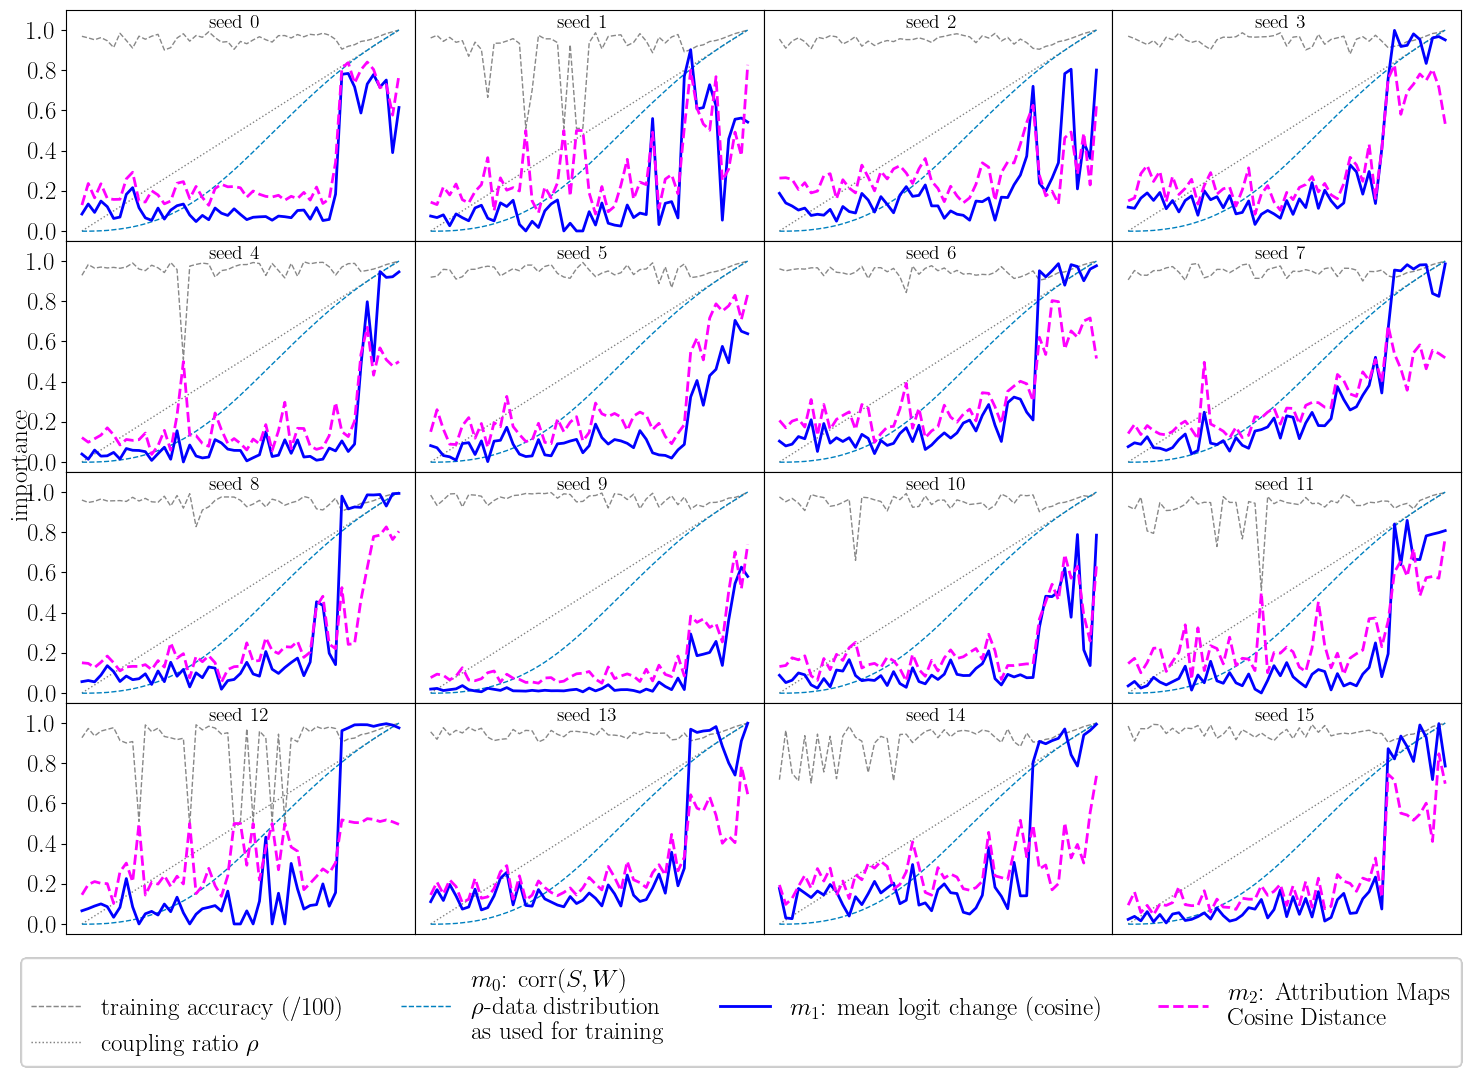
\includegraphics[width=\textwidth]{thesis_latex_template/pics/compare_seeds_overlap.png}
	\caption[Pattern Scenario Compare Seeds]{Comparing ground truth importance over 10 random initializations}
\end{figure}

\begin{figure}[!htb]
    \centering
    \includegraphics[width=1\linewidth]{thesis_latex_template/pics/mac_measures_overlap.png}
    \caption{Mean Attribution Change measures (with different distance metrics)  }
    \label{fig:mac_measures_overlap}
\end{figure}

\section{Additional Figures}

\begin{figure}[!htb]
	\centering
	\label{fig:some_more}
	\includegraphics[width=\textwidth]{thesis_latex_template/pics/scatter_plot_matrix.png}
	\caption[Test]{Scatter plots for the 4 different ground truth measures $m_1$ and all different explanation importance measures $m_2$ for Watermark Scenario}
\end{figure}

\begin{figure}[!htb]
    \centering
    \includegraphics[width=1\linewidth]{thesis_latex_template/pics/r2_m1_vs_m2.png}
    \caption{R2 score between ground truth $m_1$ (mean absolute distance) and measure $m_2$ for Watermark Scenario}
\label{fig:enter-label}
\end{figure}

\begin{figure}[!htb]
    \centering
    \includegraphics[width=1\linewidth]{thesis_latex_template/pics/mse_attribution_per_m2.png}
    \caption{Mean Square Error between explanation importance measure and true importance $m_1$ for Watermark Scenario}
    \label{fig:enter-label}
\end{figure}


\begin{figure}[!htb]
	\centering
	\label{fig:some_more}
	\includegraphics[width=\textwidth]{thesis_latex_template/pics/scatter_plot_matrix_overlap.png}
	\caption[Test]{Scatter plots for the 4 different ground truth measures $m_1$ and all different explanation importance measures $m_2$ for pattern Scenario}
\end{figure}

\begin{figure}[!htb]
    \centering
    \includegraphics[width=1\linewidth]{thesis_latex_template/pics/r2_m1_vs_m2_overlap.png}
    \caption{R2 score between ground truth $m_1$ (mean absolute distance) and measure $m_2$ for pattern Scenario}
\label{fig:enter-label}
\end{figure}

\begin{figure}[!htb]
    \centering
    \includegraphics[width=1\linewidth]{thesis_latex_template/pics/mse_attribution_per_m2_overlap.png}
    \caption{Mean Square Error between explanation importance measure and true importance $m_1$ for pattern Scenario}
    \label{fig:enter-label}
\end{figure}